\subsection*{Figures}

\begin{figure}[ht!]
    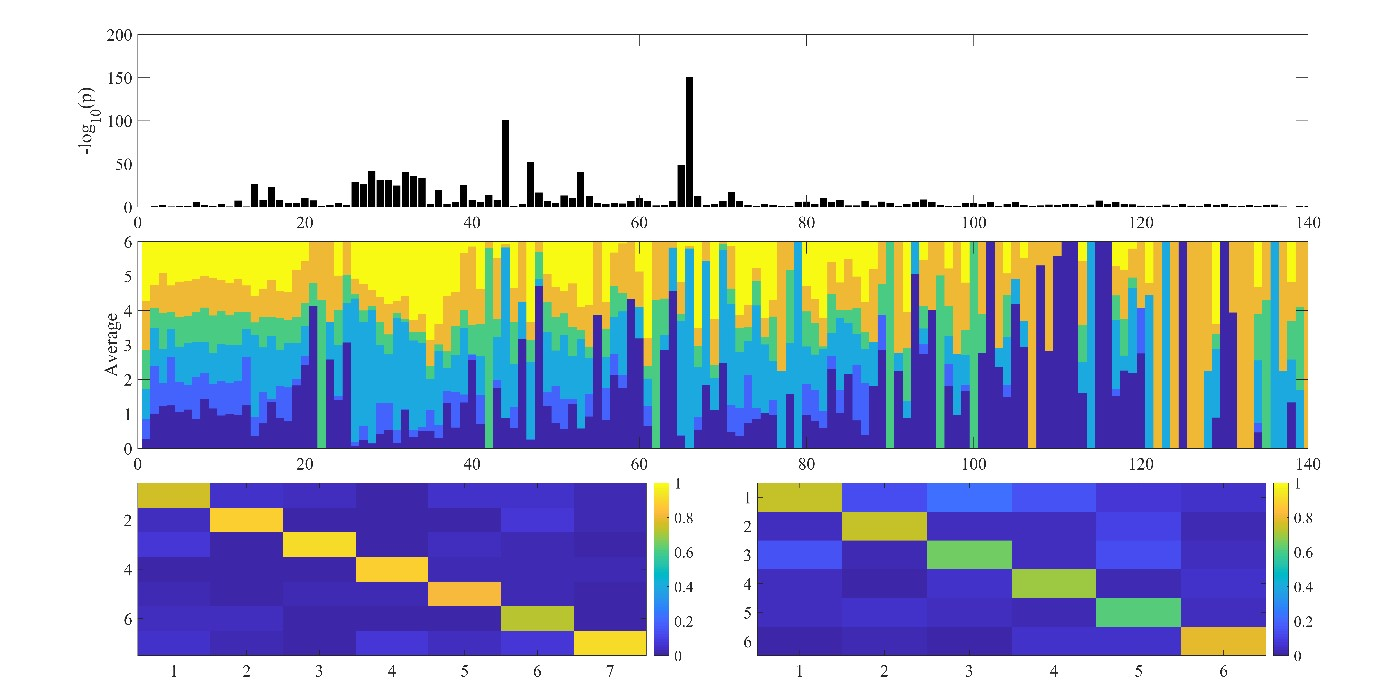
\includegraphics[width=\textwidth]{kruskal.jpg}
    \centering
    \caption{
        \textit{
            \\A)  $Log(p)$ value of non-parametric Kruskal Wallis test for the association of each topological feature with the class of the manuscripts in CiteSeer. The $x-axis$ is the feature number (Table \ref{tab:dataset}). One can see that some features are highly associated with the manuscript class.
            \\B)  Average of each topological feature for nodes belonging to a given class. All values were stacked and normalized to 1. An equal distribution would produce equally divided columns.
            \\C)  Correlation of CiteSeer and Cora manuscript class with the neighboring manuscript class. The color in each row represents the fraction of nodes neighboring a given class that belong to all possible classes. One can see the dominating diagonal representing the fact that neighboring nodes tend to have the same color. However, when the topology is incorporated, an even more accurate estimate of the node color can be obtained.
        }
    }
    \label{fig:kruskal}
\end{figure}


\begin{figure}[ht!]
    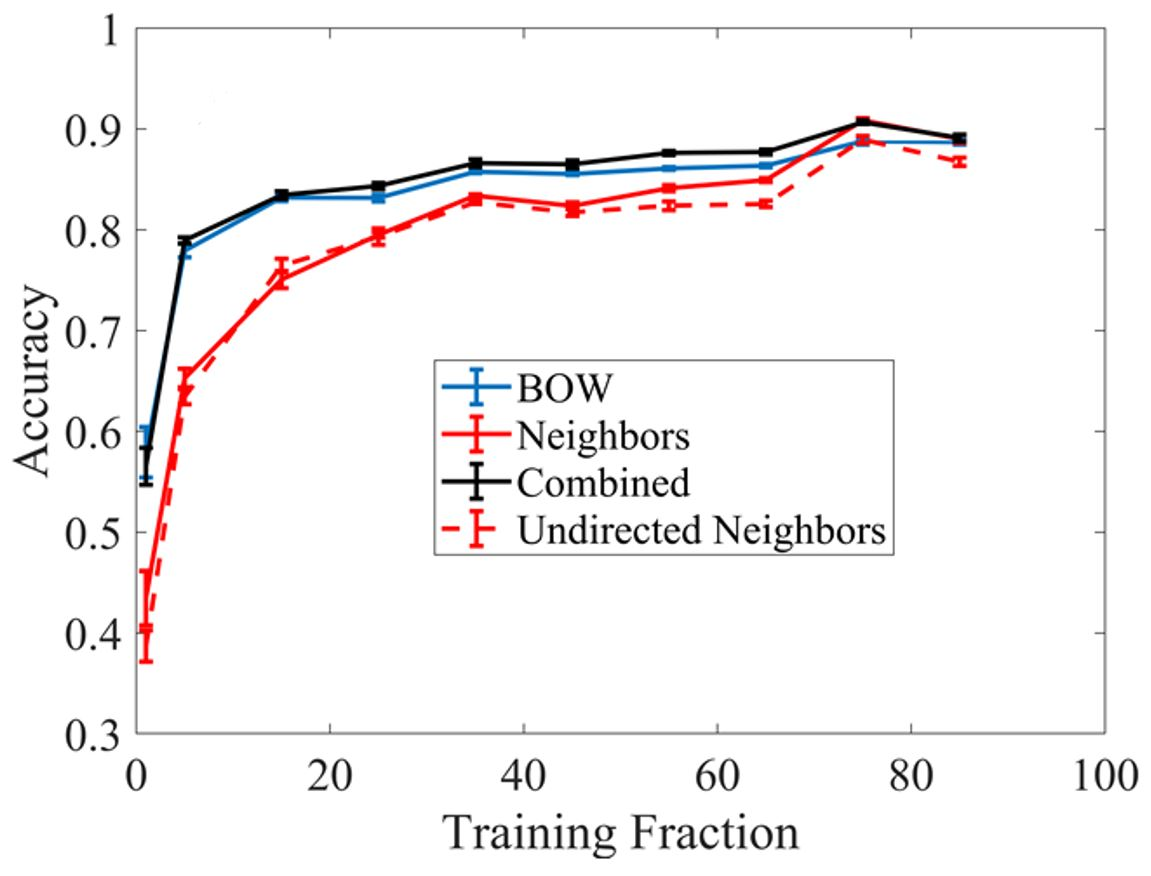
\includegraphics[width=0.7\textwidth]{acc_percentage2.JPG}
    \centering
    \caption{\textit{
        Comparison between the current state of the art (full dark line), our combined method (dashed-dotted blue line), the same method when the only topology is used (green dashed and red dotted lines). The dashed line is for the asymmetric network, while the red line is for the symmetric network. The $y-axis$ is the test accuracy and the $x-axis$ is the training set fraction.
        }}
    \label{fig:acc_comp}
\end{figure}


\begin{figure}[ht!]
    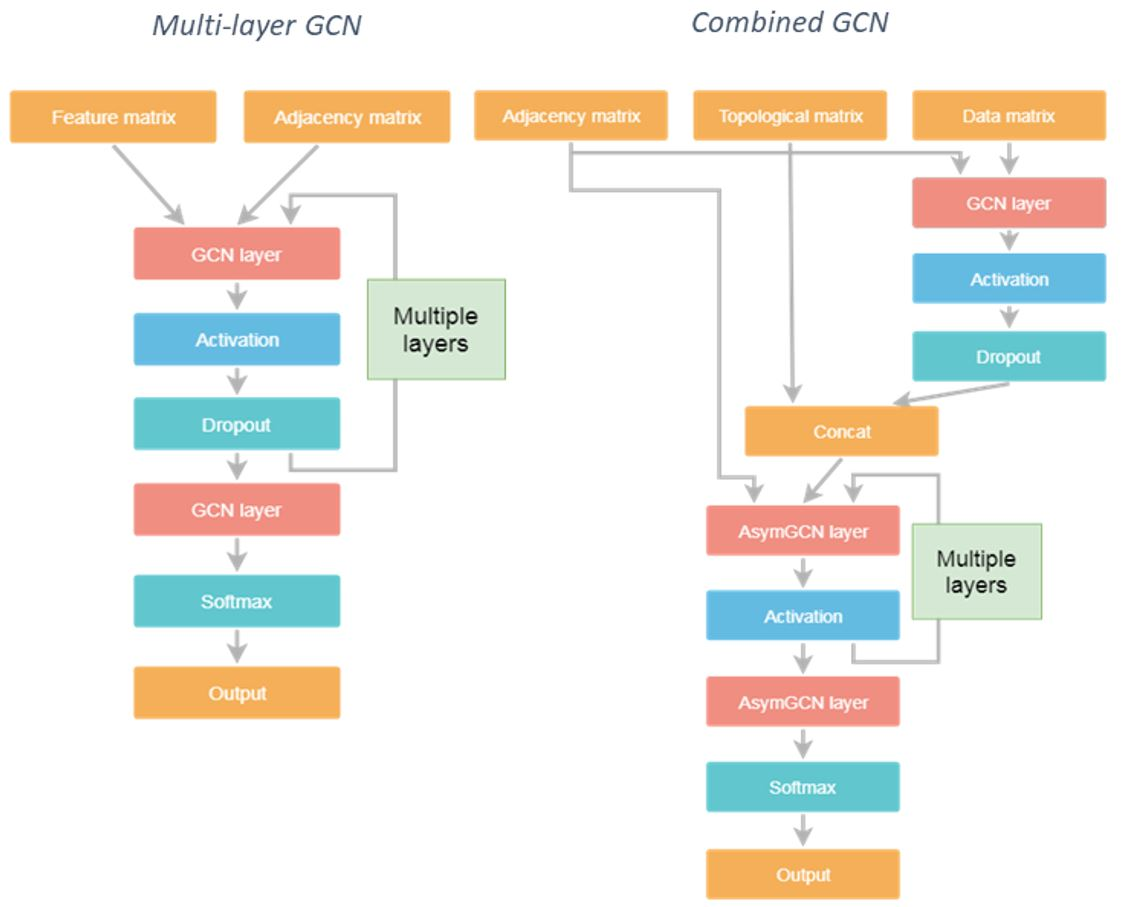
\includegraphics[width=0.7\textwidth]{models2.jpg}
    \centering
    \caption{\textit{
        Network descriptions. Left side network GCN based on neighbor classification/topology. The network classification or topology is used as an input and the multiple GCN with either symmetric or full asymmetric networks are used. The nonlinearity in each internal layer is a ReLu, and the output nonlinearity is a softmax when this is combined with external information as is the case for example for the BOW (right figure). This information is passed through a first GCN layer and the output of this layer is fed to the next layers (right network).
        }}
    \label{fig:models}
\end{figure}


\begin{figure}[ht!]
    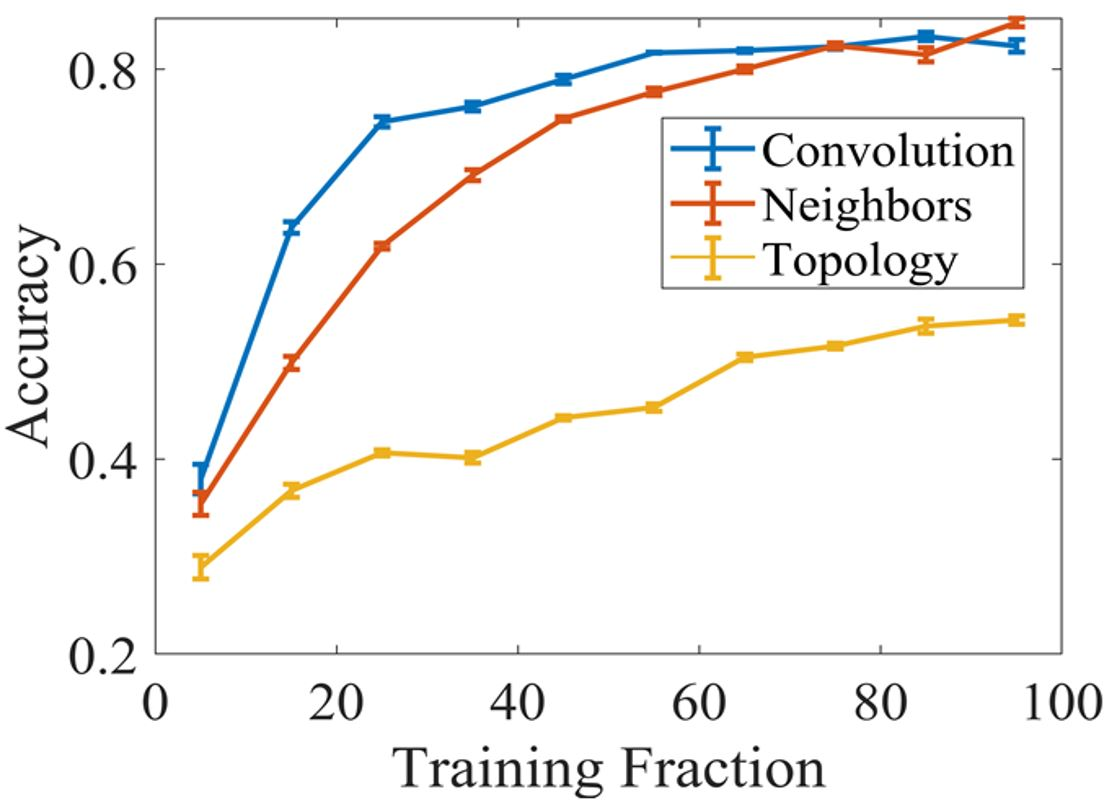
\includegraphics[width=0.7\textwidth]{acc_percentage.JPG}
    \centering
    \caption{\textit{
        Lower plot: accuracy of the CiteSeer classification can be obtained when only topological features are used. Middle plot: accuracy when each node is classified using the distribution of classes in its neighbors. Upper plot: accuracy obtained when products of the neighbors and different combinations of the adjacency matrix are used.
        }}
    \label{fig:acc_per}
\end{figure}


\begin{figure}[ht!]
    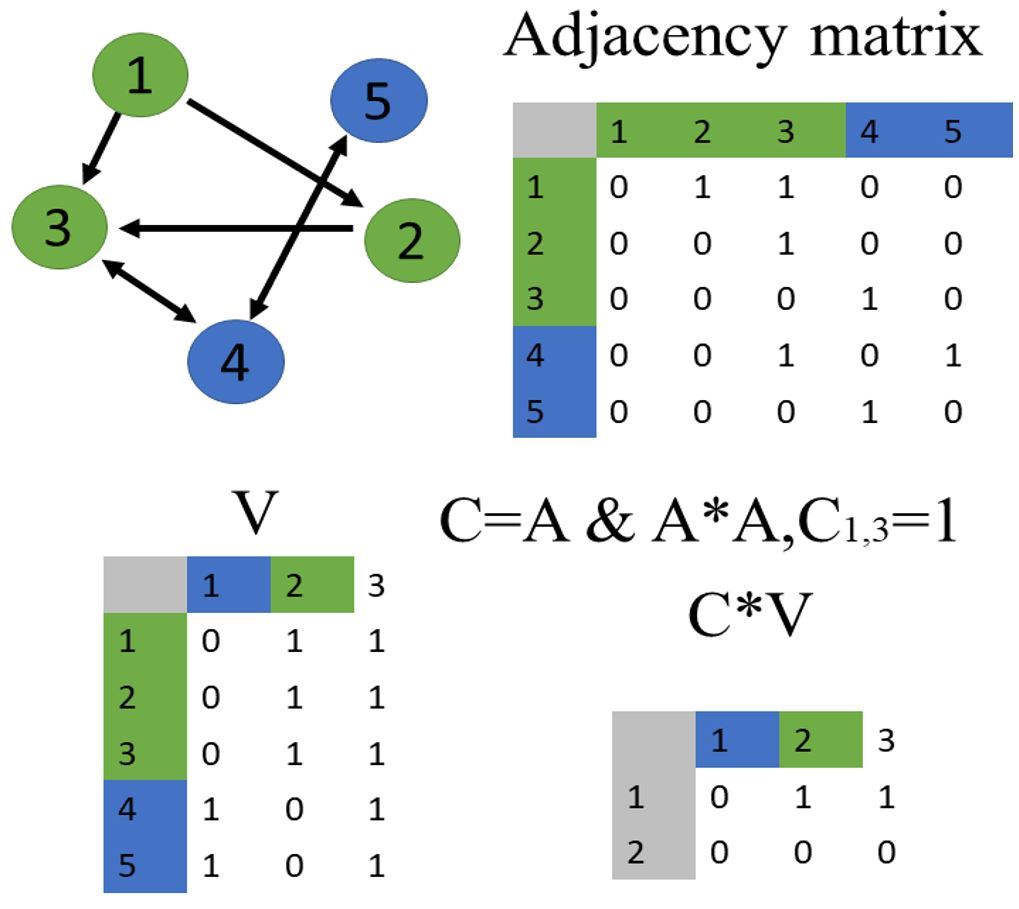
\includegraphics[width=0.7\textwidth]{adj_example.JPG}
    \centering
    \caption{\textit{
        Example of sub-graph frequency through adjacency matrix products.   Given the graph plotted on the left and the appropriate adjacency matrix ($A$), one can count the number of feed-forward motifs ($x\rightarrow y and x\rightarrow z\rightarrow y$) originating from green and blue nodes through the product of $A \& A\cdot A$ with the color one-hot matrix of the nodes ($V$). One can see that there is a total of 1 such triangle and it originates from a green node.
        }}
    \label{fig:adj_example}
\end{figure}